\chapter{Threshold voltages of the PMTs}
\label{sec:appendix}
\begin{figure}
    \centering
    \begin{subfigure}[b]{0.48\textwidth}
    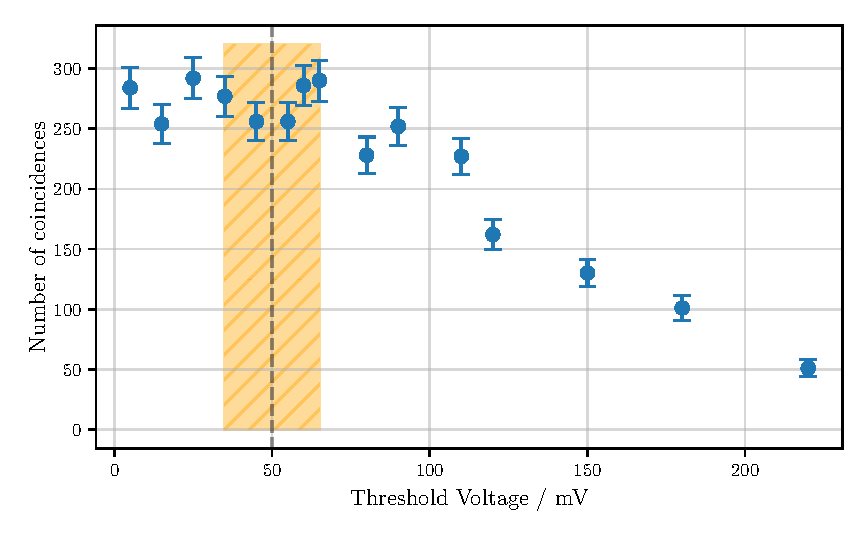
\includegraphics[width=\textwidth]{plots/threshR00.pdf}
    \captionof{figure}{Data of the \texttt{R00} signal.
    The central value of the plateau is $\SI{50}{mV}$.}
\end{subfigure}\hfill
\begin{subfigure}[b]{0.48\textwidth}
    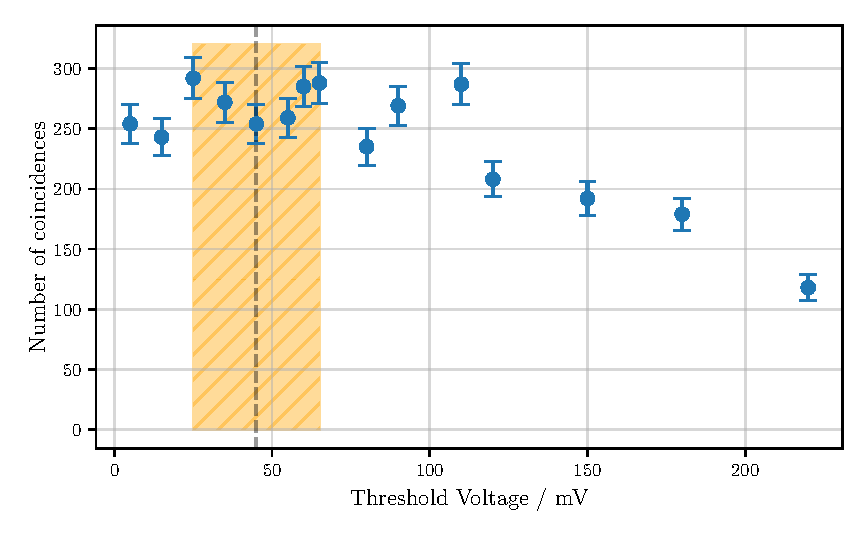
\includegraphics[width=\textwidth]{plots/threshR10_2.pdf}
    \captionof{figure}{Data of the second measurement of the \texttt{R10} signal.
    The central value of the plateau is $\SI{45}{mV}$.}
\end{subfigure}
\caption{Measured number of coincidences concerning varying threshold voltages
of the \texttt{R00} and \texttt{R10} PMTs.
The dashed line indicates the central values of each plateau. The striped orange areas mark the found plateaus.}
\label{fig:appthresh1}
\end{figure}
\begin{figure}
    \begin{subfigure}[b]{0.48\textwidth}
        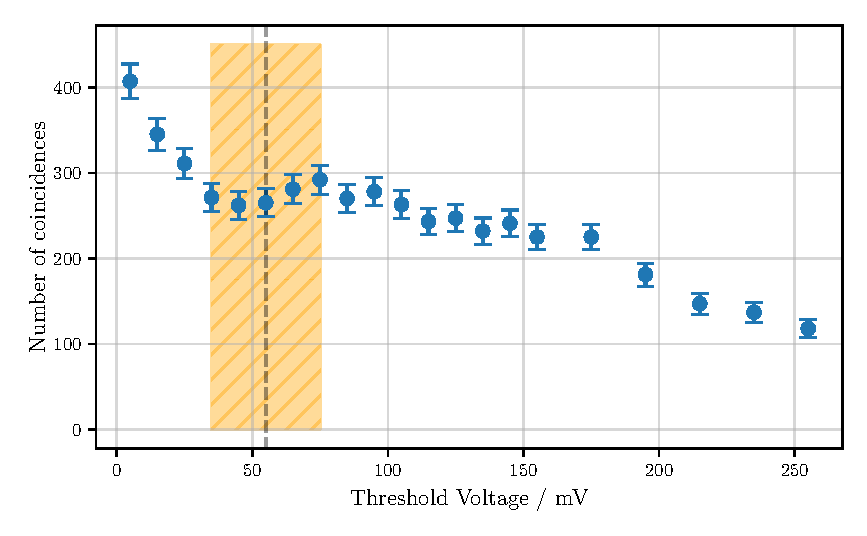
\includegraphics[width=\textwidth]{plots/threshR01.pdf}
        \captionof{figure}{Data of the \texttt{R01} PMTs.
        The central value of the plateau is $\SI{55}{mV}$.}
    \end{subfigure}\hfill
    \begin{subfigure}[b]{0.48\textwidth}
        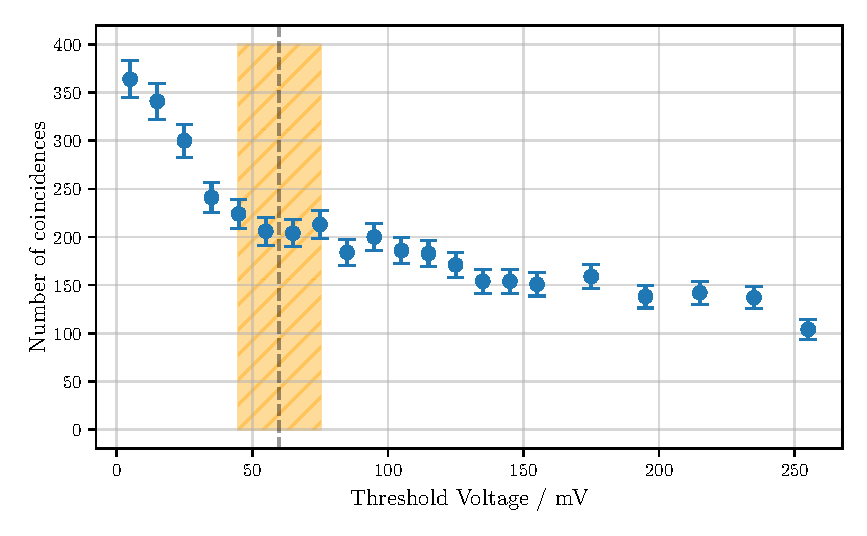
\includegraphics[width=\textwidth]{plots/threshR11.pdf}
        \captionof{figure}{Data of the \texttt{R11} PMTs.
        The central value of the plateau is $\SI{60}{mV}$.}
    \end{subfigure}
    \caption{Measured number of coincidences concerning varying threshold voltages
    of the \texttt{R01} and \texttt{R11} PMTs.
    The dashed line indicates the central values of each plateau. The striped orange areas mark the found plateaus.}
    \label{fig:appthresh2}
\end{figure}   
\begin{figure}
    \centering
    \begin{subfigure}[b]{0.48\textwidth}
        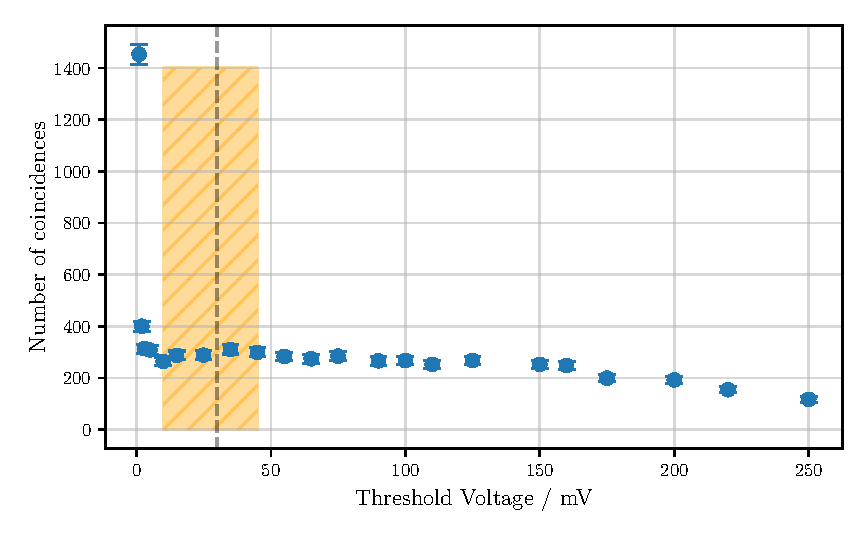
\includegraphics[width=\textwidth]{plots/threshL00.pdf}
        \captionof{figure}{Data of the \texttt{L00} PMTs.
        The central value of the plateau is $\SI{30}{mV}$.}
    \end{subfigure}\hfill
    \begin{subfigure}[b]{0.48\textwidth}
        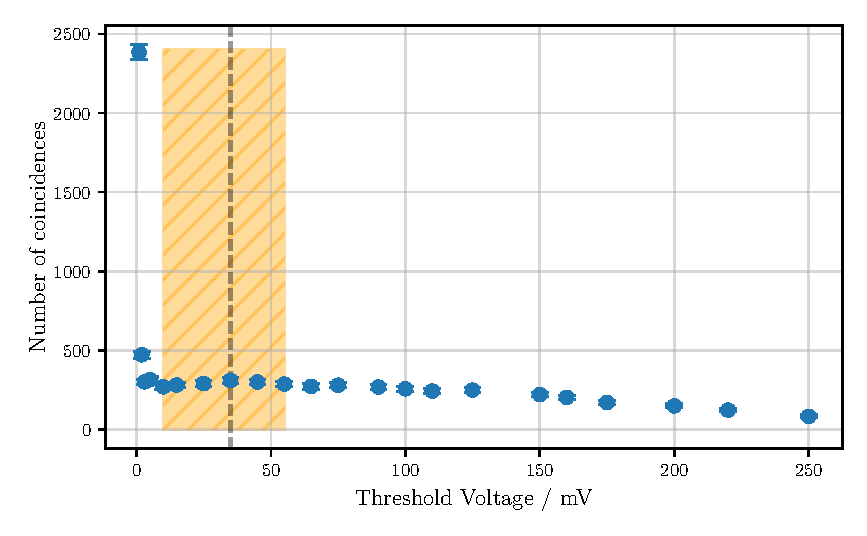
\includegraphics[width=\textwidth]{plots/threshL10.pdf}
        \captionof{figure}{Data of the \texttt{L10} PMTs.
        The central value of the plateau is $\SI{35}{mV}$.}
    \end{subfigure}
    \caption{Measured number of coincidences concerning varying threshold voltages
    of the \texttt{L00} and \texttt{L10} PMTs.
    The dashed line indicates the central values of each plateau. The striped orange areas mark the found plateaus.}
    \label{fig:appthresh3}
\end{figure}
\begin{figure}
    \centering
    \begin{subfigure}[b]{0.48\textwidth}
        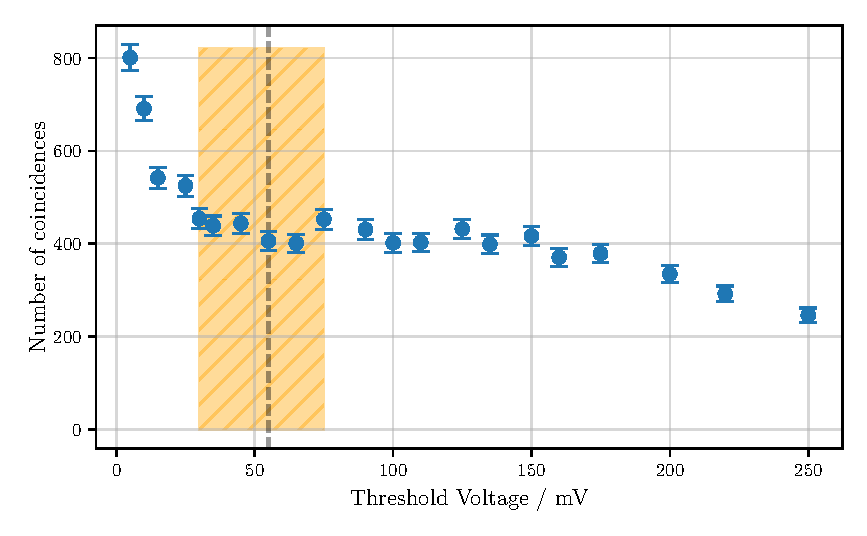
\includegraphics[width=\textwidth]{plots/threshL01.pdf}
        \captionof{figure}{Data of the \texttt{L01} PMTs.
        The central value of the plateau is $\SI{55}{mV}$.}
    \end{subfigure}\hfill
    \begin{subfigure}[b]{0.48\textwidth}
        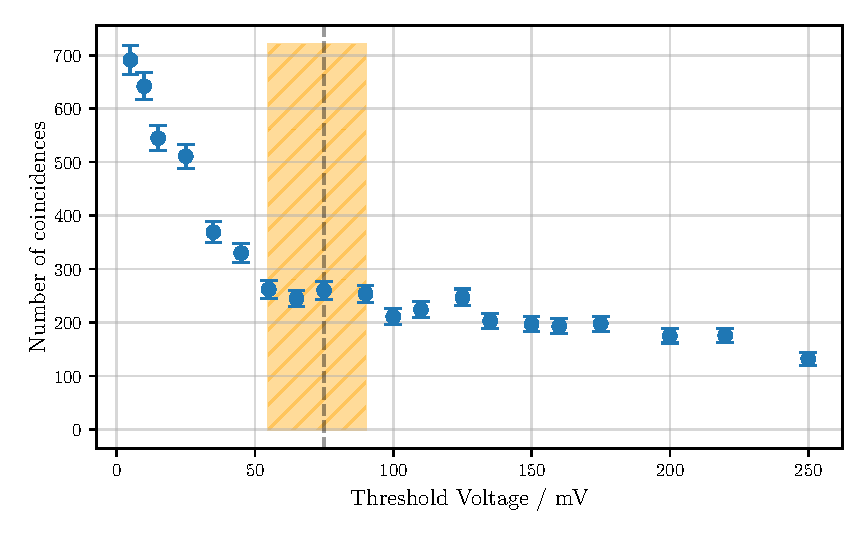
\includegraphics[width=\textwidth]{plots/threshL11.pdf}
        \captionof{figure}{Data of the \texttt{L11} PMTs.
        The central value of the plateau is $\SI{75}{mV}$.}
    \end{subfigure}
    \caption{Measured number of coincidences concerning varying threshold voltages
    of the \texttt{L01} and \texttt{L11} PMTs.
    The dashed line indicates the central values of each plateau. The striped orange areas mark the found plateaus.}
    \label{fig:appthresh4}
\end{figure}
\begin{figure}
    \centering
    \begin{subfigure}[b]{0.48\textwidth}
        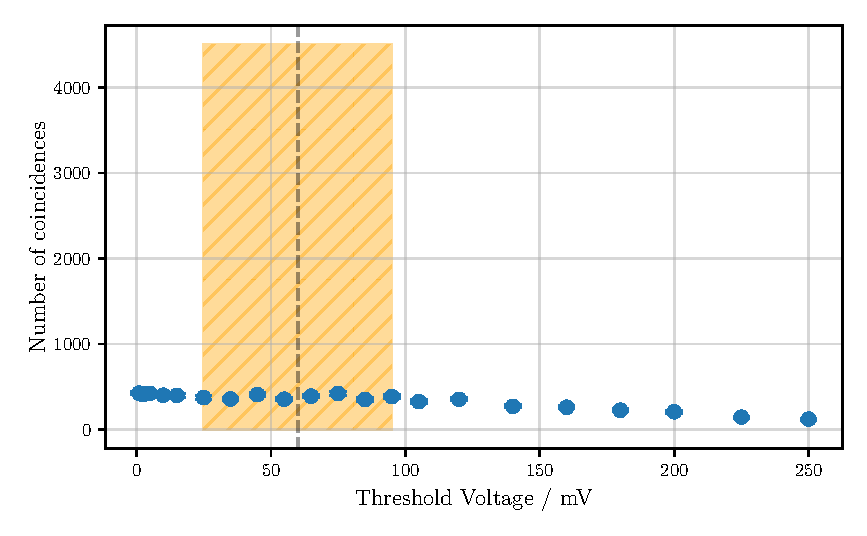
\includegraphics[width=\textwidth]{plots/threshL10_2.pdf}
        \captionof{figure}{Data of the second measurement of the \texttt{L10} PMTs.
        The central value of the plateau is $\SI{60}{mV}$.}
    \end{subfigure}\hfill
    \begin{subfigure}[b]{0.48\textwidth}
        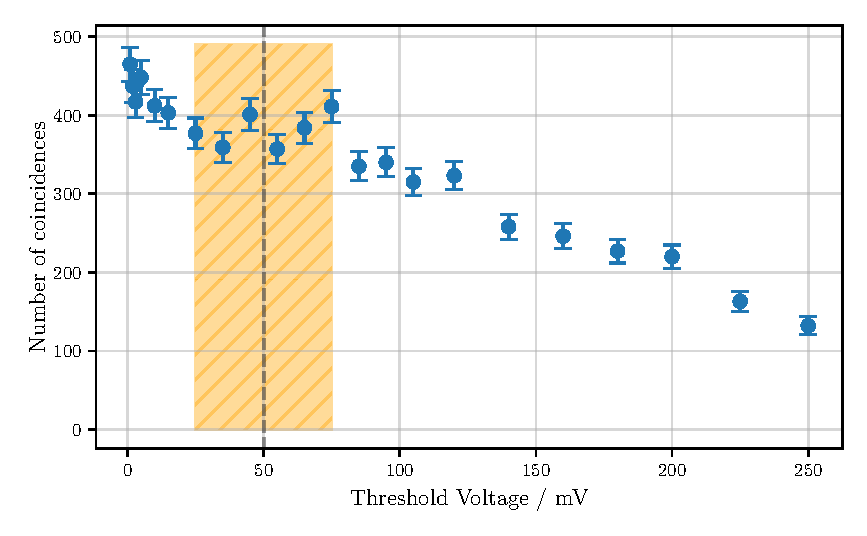
\includegraphics[width=\textwidth]{plots/threshL20.pdf}
        \captionof{figure}{Data of the \texttt{L20} PMTs.
        The central value of the plateau is $\SI{50}{mV}$.}
    \end{subfigure}
    \caption{Measured number of coincidences concerning varying threshold voltages
    of the \texttt{L10} and \texttt{L20} PMTs.
    The dashed line indicates the central values of each plateau. The striped orange areas mark the found plateaus.}
    \label{fig:appthresh5}
\end{figure}
\begin{figure}
    \centering
    \begin{subfigure}[b]{0.48\textwidth}
        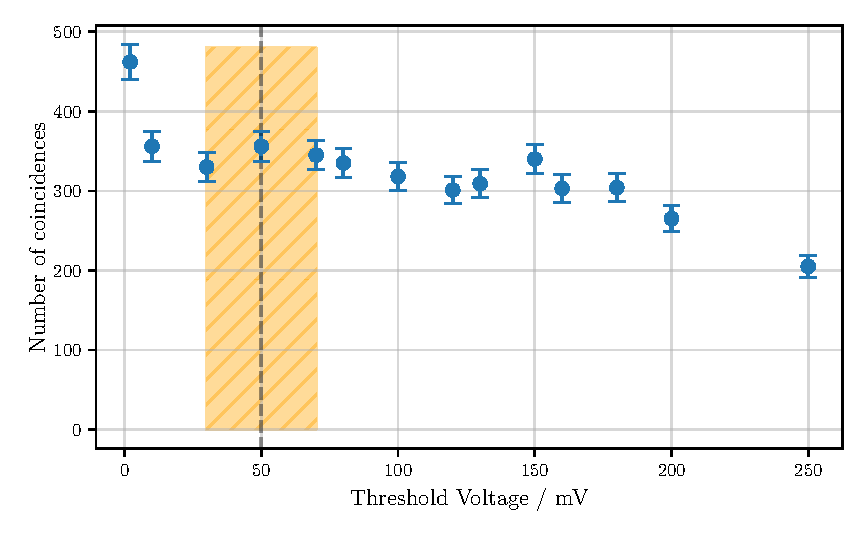
\includegraphics[width=\textwidth]{plots/threshL21.pdf}
        \captionof{figure}{Data of the \texttt{L21} PMTs.
        The central value of the plateau is $\SI{50}{mV}$.}
    \end{subfigure}\hfill
    \begin{subfigure}[b]{0.48\textwidth}
        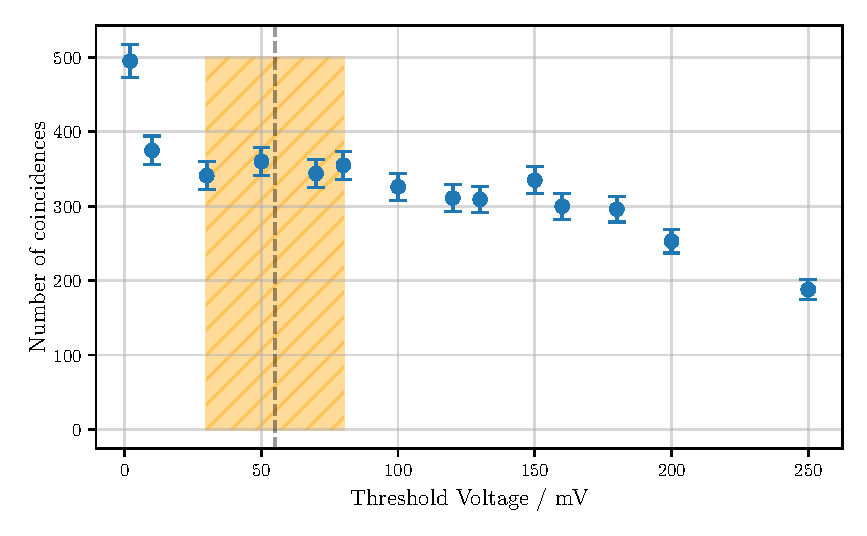
\includegraphics[width=\textwidth]{plots/threshR21.pdf}
        \captionof{figure}{Data of the \texttt{R21} PMTs.
        The central value of the plateau is $\SI{55}{V}$.}
    \end{subfigure}
    \caption{Measured number of coincidences concerning varying threshold voltages
    of the \texttt{L21} and \texttt{R21} PMTs.
    The dashed line indicates the central values of each plateau. The striped orange areas mark the found plateaus.}
    \label{fig:appthresh6}
\end{figure}
